\section{Reference aircraft}
\paragraph{} The new airport will have two runway with different Airfield reference keys. The International flights thought one, with 4E reference key and the domestic dedicated runway with 4C reference key.

New airport, will absorb around de 40\% of Soekarno-Hatta International Airport air traffic. As it can be seen, the most common code letter is C, but some big planes with code E can also appear. That is why, the new aircraft, despite it will be dedicated domestic flights, will be able to handle big international flights also, Fig. \ref{aircraftDist}.
\begin{figure}[H]
	\centering
	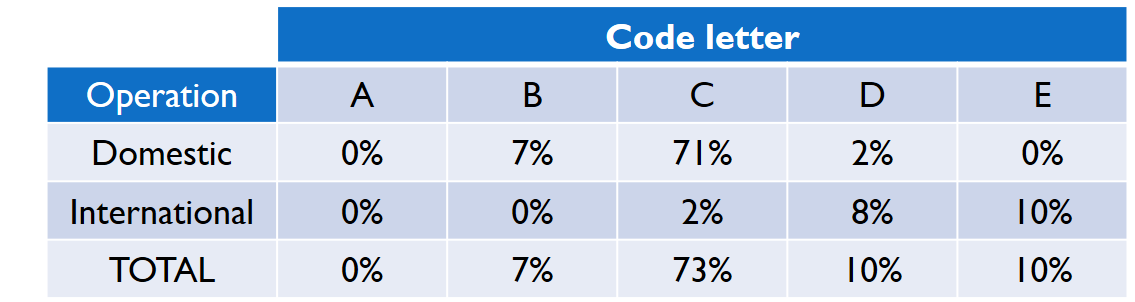
\includegraphics[clip, trim=0.1cm 0.1cm 0.1cm 0.1cm, width=0.8\textwidth]{./images/PROGNOSIS/aircraft/aircraftDist}
	\caption{Soekarno-Hatta International Airport aircraft class distribution.}
	\label{aircraftDist}
\end{figure}

	\subsection{Aircraft type for 4E reference key airfield}
	\paragraph{} A380 is discarded, because the new airport aims to absorb domestic flights mainly but also some international traffic (close range). B777-300 and A330-300, are found to be the bigger planes with higher requirements to operate on the new airport. 
	
	\subsection{Aircraft type for 4C reference key airfield}
	\paragraph{} B737-800, is chosen because have longer take-off requirements compared to A320 and other smalls planes, operating 
	
	\subsection{Conclusions}